\documentclass[a4paper, 14pt]{article}
\usepackage[utf8]{inputenc}
\usepackage[russian]{babel}
\usepackage{graphicx}
\usepackage{listings}
\usepackage{color}
\usepackage{amsmath}
\usepackage{pgfplots}
\usepackage{url}
% подключаем hyperref (для ссылок внутри  pdf)
\usepackage[unicode, pdftex]{hyperref}
\usepackage[T2A]{fontenc}
\usepackage[utf8]{inputenc}
\lstset{tabsize=2,
    breaklines,
    columns=fullflexible,
    flexiblecolumns,
    numbers=left,
    keepspaces=true,
    numberstyle={\footnotesize},
    extendedchars=\true
}
\lstdefinelanguage{MyC}{
  language=C++,
  ndkeywordstyle=\color{darkgray}\bfseries,
  identifierstyle=\color{black},
  morecomment=[n]{/**}{*/},
  commentstyle=\color{blue}\ttfamily,
  stringstyle=\color{red}\ttfamily,
  morestring=[b]",
  showstringspaces=false,
  morecomment=[l][\color{gray}]{//},
  keepspaces=true,
  escapechar=\%,
  %texcl=⟨true|false⟩
}
%\usepackage[russian,russian,english]{babel}
\frenchspacing                    % ставим пробелы в соответствии с французским стилем
\DeclareGraphicsExtensions{.pdf,.png,.jpg,.svg}
\usepackage{titlesec}
\usepackage{algpseudocode}
\usepackage{caption}
\usepackage{setspace}
\usepackage[linesnumbered,boxed]{algorithm2e}



\DeclareCaptionFont{white}{\color{white}} %% это сделает текст заголовка белым
%% код ниже нарисует серую рамочку вокруг заголовка кода.

\linespread{1}

\DeclareCaptionFormat{listing}{\colorbox{gray}{\parbox{\textwidth}{#1#2#3}}}
\captionsetup[lstlisting]{format=listing,labelfont=white,textfont=white} 

\begin{document}
	\begin{titlepage}
		\begin{center}
			\begin{LARGE}
				Отчет по лабораторной работе №7\\
					по курсу "Анализ алгоритмов"\\
					по теме "Вычислительный конвейер"
			\end{LARGE}
		
			\begin{Large}
				\vspace{10cm}
				Студент: Доктор А.А. ИУ7-53\\
					Преподаватель: Волкова Л.Л.,
								   Строганов Ю.В.\\
				
				\vspace{5cm}2018 г.				   
			\end{Large}
			
		\end{center}
		 
	\end{titlepage}

\tableofcontents
	
\newpage
\section*{Введение}
\addcontentsline{toc}{section}{Введение}
\hspace{1cm}

\default
Конве́йер — способ организации вычислений, используемый в современных процессорах и контроллерах с целью повышения их производительности (увеличения числа инструкций, выполняемых в единицу времени — эксплуатация параллелизма на уровне инструкций), технология, используемая при разработке компьютеров и других цифровых электронных устройств.

\begin{center}
\large\textbf{Описание}
\end{center}
 
\default

Конвейеризация (или конвейерная обработка) в общем случае основана на разделении подлежащей исполнению функции на более мелкие части, называемые ступенями, и выделении для каждой из них отдельного блока аппаратуры. Производительность при этом возрастает благодаря тому, что одновременно на различных ступенях конвейера выполняются несколько команд.

Идея заключается в параллельном выполнении нескольких инструкций процессора. Сложные инструкции процессора представляются в виде последовательности более простых стадий. Вместо выполнения инструкций последовательно (ожидания завершения конца одной инструкции и перехода к следующей), следующая инструкция может выполняться через несколько стадий выполнения первой инструкции. Это позволяет управляющим цепям процессора получать инструкции со скоростью самой медленной стадии обработки, однако при этом намного быстрее, чем при выполнении эксклюзивной полной обработки каждой инструкции от начала до конца \cite{conveyor_opr}.

\begin{figure}[h]
\center
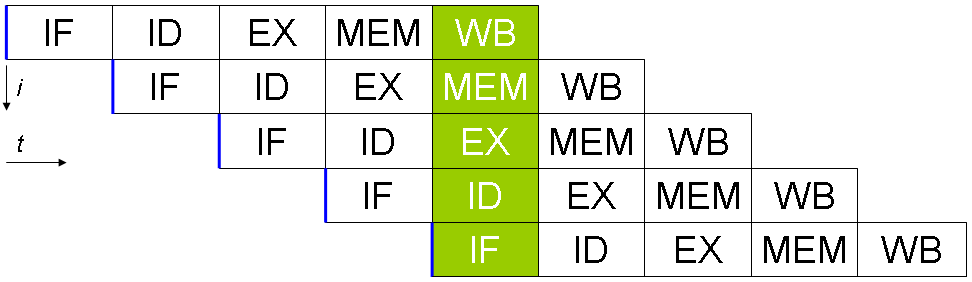
\includegraphics[scale=0.3]{risc.png}
\caption{Простой пятиуровневый конвейер в RISC-процессорах}
\label{ris:risc}
\end{figure}

На иллюстрации \ref{ris:risc} показан простой пятиуровневый конвейер в RISC-процессорах. Здесь:

\begin{enumerate}
\item[1)] IF (англ. Instruction Fetch) — получение инструкции;
\item[2)] ID (англ. Instruction Decode) — раскодирование инструкции;
\item[3)] EX (англ. Execute) — выполнение;
\item[4)] MEM (англ. Memory access) — доступ к памяти;
\item[5)] WB (англ. Register write back) — запись в регистр.
\end{enumerate}

Вертикальная ось — последовательные независимые инструкции, горизонтальная — время. Зелёная колонка описывает состояние процессора в один момент времени, в ней самая ранняя, верхняя инструкция уже находится в состоянии записи в регистр, а самая последняя, нижняя инструкция — только в процессе чтения.

\begin{center}
\large\textbf{Применение}
\end{center}
 
\default

Выполнение каждой команды складывается из ряда последовательных этапов (шагов стадий), суть которых не меняется от команды к команде. С целью увеличения быстродействия процессора и максимального использования всех его возможностей в современных микропроцессорах используется конвейерный принцип обработкии нформации. Этот принцип подразумевает, что в каждый момент времени процессор работает над различными стадиями выполнения нескольких команд, причем на выполнение каждой стадии выделяются отдельные аппаратные ресурсы. По очередному тактовому импульсу каждая команда в конвейере продвигается на следующую стадию обработки, выполненная команда покидает конвейер, а новая поступает в него \cite{conveyor_risc}.

\begin{center}
\large\textbf{Виды}
\end{center}
 
\default
Перечислим основные типы конвейеров:

\begin{enumerate}
\item[1)] Арифметический конвейер (arithmetic pipeline) — реализация в АЛУ поэтапного исполнения арифметических операций чаще всего над вещественными числами \cite{conveyor_ariph};
\item[2)] супер-конвейер, гипер-конвейер, глубокий конвейер (super-pipeline, hyper-pipeline, deep pipeline) — вычислительный конвейер с необычно большим количеством стадий. Например, процессор Intel Pentium 4 имел 20 стадий конвейера, а в модификации Prescott получил конвейер из 31 стадии \cite{conveyor_super};
\item[3)] недозагруженный конвейер (underutilized pipeline) — конвейер, в котором в одно и то же время не все стадии конвейера выполняют какую-то операцию. Например ранние процессоры MIPS имели 6-стадийный конвейер, но в каждый момент было занято только 3 его стадии.
\end{enumerate}

\newpage
\section*{Задачи работы}

В ходе выполнения данной лабораторной работы, мной были выполнены следующие задачи:

\begin{enumerate}
\item[1)] Построить вычислительный конвейер;
\item[2)] провести замеры скорости работы работы конвейера при разной нагруженности блоков.
\end{enumerate}


\newpage
\section{Аналитическая часть}
\hspace{1cm}	В данном разделе приведена оценка производительности идеального конвейера.

\subsection {Оценка производительности идеального конвейера} \\

Пусть задана операция, выполнение которой разбито на n последовательных этапов. При последовательном их выполнении операция выполняется за время

\begin{equation}\label{form:way} 
 \tau _{e}={\sum\limits_{i=1}^n \tau _{i}}
 \end{equation}
 \begin{align*}
    \text{где} \\
    n &- \text{количество последовательных этапов;} \\
   \tau _{i} &- \text{время выполнения i-го этапа;}
\end{align*}

Быстродействие одного процессора, выполняющего только эту операцию, составит

\begin{equation}\label{form:way} 
 S_{e}={\frac{1}{\tau _{e}}}={\frac{1}{\sum\limits_{i=1}^n \tau _{i}}}
 \end{equation}
 \begin{align*}
    \text{где} \\
    \tau _{e} &- \text{время выполнения одной операции;} \\
    n &- \text{количество последовательных этапов;} \\
   \tau _{i} &- \text{время выполнения i-го этапа;}
\end{align*}

Выберем время такта — величину t _{T} = max{\sum\limits_{i=1}^n(\tau_{i})}$ и потребуем при разбиении на этапы, чтобы для любого i = 1, ... , n выполнялось условие (\tau_{i}$ + \tau_{i+1}$) mod n = \tau_{T}$. То есть чтобы никакие два последовательных этапа (включая конец и новое начало операции) не могли быть выполнены за время одного такта.

Максимальное быстродействие процессора при полной загрузке конвейера составляет

\begin{equation}\label{form:way} 
 S_{max}={\frac{1}{\tau _{T}}}}
 \end{equation}
 \begin{align*}
    \text{где} \\
    \tau _{T} &- \text{выбранное нами время такта;}
\end{align*}

Число n — количество уровней конвейера, или глубина перекрытия, так как каждый такт на конвейере параллельно выполняются n операций. Чем больше число уровней (станций), тем больший выигрыш в быстродействии может быть получен.

Известна оценка
\begin{equation}\label{form:way} 
{\frac{n}{n/2} \leq {\frac{S_{max}}{S_{e}}} \leq n}
 \end{equation}
 \begin{align*}
    \text{где} \\
    S_{max} &- \text{максимальное быстродействие процессора  при полной загрузке конвейера;} \\
    S_{e} &- \text{стандартное быстродействие процессора;} \\
   n &- \text{количество этапов.}
\end{align*}

то есть выигрыш в быстродействии получается от n/2  до n раз \cite{conveyor_mark}.

Реальный выигрыш в быстродействии оказывается всегда меньше, чем указанный выше, поскольку:

\begin{enumerate}
\item[1)] некоторые операции, например, над целыми, могут выполняться за меньшее количество этапов, чем другие арифметические операции. Тогда отдельные станции конвейера будут простаивать;
\item[2)] при выполнении некоторых операций на определённых этапах могут требоваться результаты более поздних, ещё не выполненных этапов предыдущих операций. Приходится приостанавливать конвейер;
\item[3)] поток команд(первая ступень) порождает недостаточное количество операций для полной загрузки конвейера.
\end{enumerate}
	
		\newpage
	\section{Конструкторская часть}
	\hspace{1cm}В данном разделе будут описаны принципы работы выбранных решений и их блоксхемы.
	\subsection{Разработка реализаций алгоритмов}
	
\hspace{1cm} Моя программа "собирает" танки из трёх компонентов: корпуса, двигателя и пушки. Итого 3 этапа сборки. Один этап представлена классом TankQueue, который хранит следующие поля:
	\begin{enumerate}
	\item[1)] tanks - Очередь танков, ожидающих выполнения действия;
    \item[2)] work - функтор - функция постройки;
    \item[3)] queue\_mutex - временной(для установки времени ожидания) мьютекс для блокировки доступа к очереди выполнения;
    \item[4)] main - флаг первой активной очереди;
    \item[5)] build\_time - время постройки;
    \item[6)] downtime - время ожидания появления элементов в очереди;
    \item[7)] time\_for\_mutex - время ожидания на мьютексе;
    \item[8)] id - идентификатор танка для отладки.
    \end{enumerate}
    
    Я упомянул очередь танков. Под танками я подразумеваю класс Tank с разными методами сборки(в них нет ничего интересного, они будут приведены ниже в соответсвующем листинге). Единственное важное, что у танка тоже есть свой мьютекс - tank\_mutex.
    
    Итак, как работает мой конвейер. Создаются 5 очередей TankQueue. В конвейере 3 составляющих, а очередей 5, почему так? 2 очереди отведены просто под хранилища танков: первоначальные танки(пустые) и конечные(полностью построенные). Оставшиеся три предназначены для установки корпуса, двигателя и пушки. Всем очередям присваивается флаг конца работы False. Очередь пустых танков является первой очередью, поэтому ее флаг main устанавливается в True. В очередь готовых к исполнению танков для класса TankQueue пустых танков заносится очередь из 5 танков. Всё, на этом приготовления закончены. Все составляющие конвейера готовы к работе. Танк считается построенным, если он получил корпус, двигатель и пушку - см. рис. \ref{ris:build}
    
    \begin{figure}[h!]
    \center
    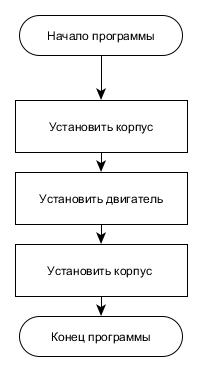
\includegraphics[scale=0.8]{tank_build.jpg}
    \caption{Алгоритм построения танка}
    \label{ris:build}
    \end{figure}\newpage
    
    Запускаем потоки для каждой очереди. Функцией потока выбирается метод start, принимающий на вход ссылку на следующую очередь. Принцип ее работы изображен на рис. \ref{ris:start1} и рис. \ref{ris:start2}. Функция постоянно ожидает, когда флаг конца работы(finish) станет True. Если же он False, то функция смотрит, хранится ли в очереди ее класса какие нибудь танки, которые надо обработать. Если да, то захватываем мьютекс очереди выполнения, достаём первый танк и освобождаем мьютекс. Далее выполняем работу над танком. Помните функтор work? Вот его и вызываем. Ему на вход требуется танк и время выполнения. Танк есть, а время выполнения хранится в build_$time. Его принцип работы изображен на рис. \ref{ris:component}.
    
     \begin{figure}[h!]
    \center
    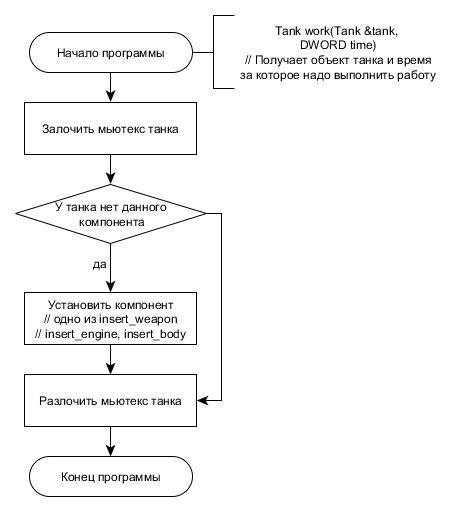
\includegraphics[scale=0.6]{component_thread.jpg}
    \caption{Установка компонента в танк}
    \label{ris:component}
    \end{figure}\newpage
    
    После того как работа выполнена пытаемся подключить к очереди следующего этапа конвейера. Ожидаем на мьютексе следующей очереди time\_for\_mutex секунд. Если подключиться не удается засыпаем на некоторое время, чтобы подождать освобождения мьютекса. Этот цикл закончится только после того, как мы достигнем нашей цели и захватим мьютекс. Как только мы его захватываем, мы кладем в конец очереди обработанный нами танк и освобождаем мьютекс. Так мы крутимся в нашей очереди выполнения, пока она не опустеет. Как только она опустеет, выходим из нее и смотрим, является ли данный класс главный этапом конвейера. Если да, то еще раз убеждаемся, что очередь пустая. Под главным этапом я подразумеваю такой этап, в который нельзя послать новые элементы, поскольку он является первым. Итак, если текущий этап таковой и его очередь пуста, то назначаем следующий этап главным, а у себя ставим флаг finish в True - то есть прекращаем работу. Если же текущий этап не являлся не главным, то засыпаем на время downtime, ожидая, пока в нашу очередь добавят новых танков. После чего просыпаемся и по новой. Сигнал завершения был? Нет? Тогда пока очередь не пуста, обрабатываем нашу очередь, занося обработанные танки в следующую и надеемся, что нашу очередь сделали главной и мы можем прекратить работу и пойти отдыхать, назначив главной следующую. А теперь тоже самое, но в виде схемы - рисунки \ref{ris:start1}, \ref{ris:start2}.
    
    \begin{figure}[h!]
    \center
    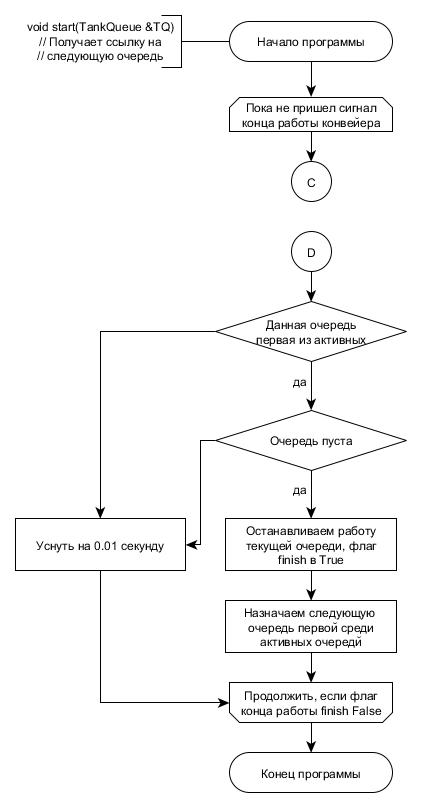
\includegraphics[scale=0.65]{start_part1.jpg}
    \caption{Цикл работы, пока не наступил флаг конца работы.}
    \label{ris:start1}
    \end{figure}\newpage
    
    \begin{figure}[h!]
    \center
    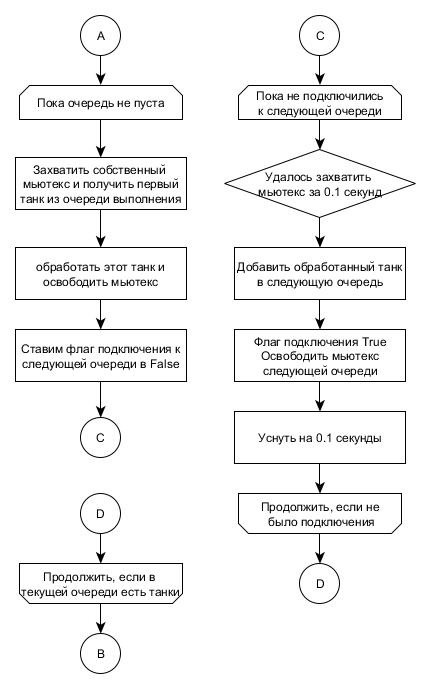
\includegraphics[scale=0.65]{start_part2.jpg}
    \caption{Обработка танка и добавление его в следующую очередь.}
    \label{ris:start2}
    \end{figure}\newpage
    

	\newpage
	\section{Технологическая часть}
	\hspace{1cm}В данном разделе будут определены средства реализации и приведен листинг кода.
	

	\subsection{Средства реализации}
	\hspace{1cm}Не изменяю себе и вновь использую C++.
	Среда разработки - Qt.
	Время работы процессора замерялось с помощью функции, продемонстрированной в листинге \ref{time}. Эта функция в отличие от встроенной функции таймера, способна считать реальное процессорное время работы программы в тиках \cite{lom}. Для ее работы была подключена библиотека time.h. Для работы с потоками и мьютексами применялись библиотеки windows.h(Для сна Sleep), mutex, thread. Контейнером очереди был std::queue, поэтому также использовалась библиотека queue.
	\lstset{ %
        language=c++,                 % выбор языка для подсветки (здесь это С)
        basicstyle=\small\sffamily, % размер и начертание шрифта для подсветки кода
        numbers=left,               % где поставить нумерацию строк (слева\справа)
        numberstyle=\tiny,           % размер шрифта для номеров строк
        stepnumber=1,                   % размер шага между двумя номерами строк
        numbersep=-5pt,                % как далеко отстоят номера строк от         подсвечиваемого кода
        backgroundcolor=\color{white}, % цвет фона подсветки - используем         \usepackage{color}
        showspaces=false,            % показывать или нет пробелы специальными     отступами
        showstringspaces=false,      % показывать или нет пробелы в строках
        showtabs=false,             % показывать или нет табуляцию в строках
        frame=single,              % рисовать рамку вокруг кода
        tabsize=2,                 % размер табуляции по умолчанию равен 2 пробелам
        captionpos=t,              % позиция заголовка вверху [t] или внизу [b] 
        breaklines=true,           % автоматически переносить строки (да\нет)
        breakatwhitespace=false, % переносить строки только если есть пробел
        escapeinside={\%*}{*)},   % если нужно добавить комментарии в коде
	    keywordstyle=\color{blue}\ttfamily,
	    stringstyle=\color{red}\ttfamily,
	    commentstyle=\color{green}\ttfamily,
	    morecomment=[l][\color{magenta}]{\#},
	    columns=fullflexible
    }
	\begin{lstlisting}[label=time,caption=Функция замера процессороного времени]
    unsigned long long tick(void)
    {
        unsigned long long d;
        __asm__ __volatile__ ("rdtsc" : "=A"     (d));
        return d;
    }
	\end{lstlisting}

	\newpage
	\subsection{Реализация алгоритмов}
	
	Как я упомянал в конструкторской части, были написаны классы Tank(листинг \ref{code:tank}) и TankQueue(листинг  \ref{code:TankQueue}). 
		\begin{lstlisting}[label=code:tank,caption=Класс Tank]
        class Tank : public Unit
        {
        public:
            static int count;
            int id;
            std::mutex tank_mutex;
        
            Tank(){id = Tank::count++; built = false;}
             ~Tank(){}
        
            void insert_weapon(Weapon weapon, DWORD time) {
                Sleep(time);
                _weapon = weapon;
            }
        
            void insert_body(Body body, DWORD time) {
                Sleep(time);
                _body = body;
            }
        
            void insert_engine(Engine engine, DWORD time) {
                Sleep(time);
                _engine = engine;
            }
        
            bool has_engine(){return _engine.is_built();}
            bool has_weapon(){return _weapon.is_built();}
            bool has_body(){return _body.is_built();}
        
            bool is_ready() {return _engine.is_built() && _body.is_built() && _weapon.is_built();}
        
            bool is_built() {return built;}
        
        
            void complete() {
                if (_engine.is_built() && _body.is_built() && _weapon.is_built()) {
                    Sleep(50);
                    built = true;
                }
            }
        
            // Конструктор копирования для queue.pop
            Tank(const Tank & other) {
                _engine = other._engine;
                _body = other._body;
                _weapon = other._weapon;
                id = other.id;
            }
        
            Tank & operator=(const Tank & other) {
                _engine = other._engine;
                _body = other._body;
                _weapon = other._weapon;
                id = other.id;
        
                return *this;
            }
        
            void move(int speed);
            void rotate(double angle);
            void fire();
        
        private:
            bool built;
            Engine _engine;
            Body _body;
            Weapon _weapon;
        };
    	\end{lstlisting}
    	
    		\begin{lstlisting}[label=code:TankQueue,caption=Класс TankQueue]
        class TankQueue {
    private:
        // Очередь готовых на выполнение
        std::queue<Tank> tanks;
        // Функтор - функция постройки
        std::function<Tank(Tank &tank, DWORD time)> work;
        // Мьютекс для блокировки доступа к очереди выполнения
        std::timed_mutex queue_mutex;
        // флаг конца работы, можно было сделать без него, но так понятнее
        bool finish;
        // флаг первого рабочего конвейера
        bool main;
    public:
        // Время ожидания на мьютексе
        DWORD time_for_mutex;
        // Время ожидания появления элементов в очереди
        DWORD downtime;
        // время постройки - занесено сюда для тестирования
        DWORD build_time;
        // идентификатор танка - занесен сюда для отладки
        int id;
        // статическая переменаня нужна для id
        static int count;
    
        // Конструкторы копирования и перемещения
        TankQueue(const TankQueue & other);
    
        TankQueue(const TankQueue && other);
    
        // Для очереди функций работы с танками
        TankQueue(std::function<Tank(Tank&, DWORD)> f, DWORD t);
    
        // Для очереди готовых танков
        TankQueue(){} // не использовать больше нигде
    
        // Для очереди пустых танков
        TankQueue(size_t amount);
    
        void set_main() {
            main = true;
        }
    
        void start(TankQueue &TQ);
    
        Tank pop() {
            Tank tank = tanks.front();
            tanks.pop();
            return tank;
        }
    
        void push(Tank &tank) {
            tanks.push(tank);
        }
    
        size_t size() {
            return tanks.size();
        }
    };
	\end{lstlisting}
	
    Кода как всегда много, поэтому для упрощения маршрутизации по отчету, приведу здесь гиперссылки по оставшимся листингам. Нумерация от наиболее важных функций к второстепенным:
    \begin{enumerate}
	\item[листинг \ref{code:start}] \hyperref[code:start]{ -& start};

    \item[листинг \ref{code:add_engine}]  \hyperref[code:add_engine]{ -& add\_engine};
    
    \item[листинг \ref{code:add_weapon}] \hyperref[code:add_weapon]{ -& add\_weapon};
    
     \item[листинг \ref{code:add_body}] \hyperref[code:add_body]{ -& add\_body};
     
     \item[листинг \ref{code:main}] \hyperref[code:main]{ -& main};
    
    \item[листинг \ref{code:TankQueue1}] \hyperref[code:TankQueue1]{ -& конструктор класса для пустой очереди};
    
    \item[листинг \ref{code:TankQueue2}] \hyperref[code:TankQueue2]{ -& конструктор класса для очереди строительства};
   
   \item[листинг \ref{code:TankQueue3}] \hyperref[code:TankQueue3]{ -& конструктор копирования};
   
    \item[листинг \ref{code:TankQueue4}] \hyperref[code:TankQueue4]{ -& конструктор перемещения};
    
    \item[листинг \ref{code:Body}] \hyperref[code:Body]{ -& класс Body};
    
    \item[листинг \ref{code:Engine}] \hyperref[code:Engine]{ -& класс Engine};
    
    \item[листинг \ref{code:Weapon}] \hyperref[code:Weapon]{ -& класс Weapon};
    
     \item[листинг \ref{code:extra}] \hyperref[code:extra]{ -& дополнительные классы и определение статических переменных}.
    \end{enumerate}
	
 \begin{lstlisting}[label=code:start,caption=Функция start.]
   void TankQueue::start(TankQueue &TQ){
        finish_mutex.lock();
    
        while (!finish) {
            finish_mutex.unlock();
            queue_mutex.lock();
            while (tanks.size() > 0) {
                times_in.push_back(clock());
                Tank tank = pop();
                queue_mutex.unlock();
                tank = work(tank, build_time);
                bool connect = 0;
                while (!connect) {
                    if (TQ.queue_mutex.try_lock_for(
                                Ms(time_for_mutex))) {
                               TQ.push(tank);
                               times_out.push_back(clock());
                               connect = 1;
                               TQ.queue_mutex.unlock();
                    }
                    std::this_thread::sleep_for(Ms(50));
                }
                queue_mutex.lock();
            }
            queue_mutex.unlock();
            main_mutex.lock();
            if (main && tanks.size() == 0) {
                main_mutex.unlock();
    
                finish_mutex.lock();
                finish = 1;
                finish_mutex.unlock();
    
                TQ.main_mutex.lock();
                TQ.set_main();
                TQ.main_mutex.unlock();
    
    
                end = clock();
            } else {
                main_mutex.unlock();
                std::this_thread::sleep_for(Ms(downtime));
            }
            finish_mutex.lock();
        }
        //std::cout << "\nfinish";
        finish_mutex.unlock();
    }
	\end{lstlisting}
	
	 \begin{lstlisting}[label=code:add_engine,caption=Функция add\_engine - встроить двигатель.]
   Tank add_engine(Tank &tank, DWORD time) {
        tank.tank_mutex.lock();
    
        if (!tank.has_engine()) {
            Engine engine;
            tank.insert_engine(engine, time);
            std::cout << "\n add engine to tank " << tank.id;
        }
    
        tank.tank_mutex.unlock();
    
        return tank;
    }
	\end{lstlisting}
	
	\begin{lstlisting}[label=code:add_weapon,caption=Функция add\_weapon - встроить оружие.]
    Tank add_weapon(Tank &tank, DWORD time) {
        tank.tank_mutex.lock();
    
        if (!tank.has_weapon()) {
            Weapon weapon;
            tank.insert_weapon(weapon, time);
            std::cout << "\n add weapon to tank " << tank.id;
        }
    
        tank.tank_mutex.unlock();
    
        return tank;
    }
	\end{lstlisting}
	
	\begin{lstlisting}[label=code:add_body,caption=Функция add\_body - встроить корпус.]
      Tank add_body(Tank &tank, DWORD time) {
        tank.tank_mutex.lock();
    
        if (!tank.has_body()) {
            Body body;
            tank.insert_body(body, time);
            std::cout << "\n add body to tank " << tank.id;
        }
        tank.tank_mutex.unlock();
        return tank;
    }
	\end{lstlisting}
    
    \begin{lstlisting}[label=code:main,caption=Функция main.]
   int main()
    {
        Tank::count = 1;
        TankQueue::count = 1;
    
        size_t amount = 5;
        TankQueue tanks(amount);
    
        TankQueue queue_engine(add_engine, 90);
        TankQueue queue_body(add_body, 30);
        TankQueue queue_weapon(add_weapon, 200);
    
        TankQueue ready_tanks;
    
        std::thread give_to_body([&tanks, &queue_body](){ tanks.start(queue_body);});
        std::thread give_to_engine([&queue_body,
        &queue_engine](){
            queue_body.start(queue_engine);
            });
            
        std::thread give_to_weapon([&queue_engine,
        &queue_weapon](){
            queue_engine.start(queue_weapon);
            });
            
        std::thread give_to_ready([&queue_weapon,
        &ready_tanks](){
            queue_weapon.start(ready_tanks);
            });
    
        give_to_body.join();
        give_to_engine.join();
        give_to_weapon.join();
        give_to_ready.join();
        
        std::cout << "\n\ni finished! " << ready_tanks.size() << " " << queue_weapon.size() <<  queue_engine.size() << queue_body.size();
    
        return 0;
    }
	\end{lstlisting}
    
    \begin{lstlisting}[label=code:TankQueue1,caption=Функция TankQueue(size\_t amount) - конструктор класса для пустой очереди.]
    TankQueue::TankQueue(size_t amount){
        id = TankQueue::count++;
        for (size_t i = 0; i < amount; i++) {
            Tank tank;
            tanks.push(tank);
        }
        main = 1;
        finish = 0;
        work = noWork;
        time_for_mutex = 100;
        downtime = 10;
    }
	\end{lstlisting}
	
	\begin{lstlisting}[label=code:TankQueue2,caption= Конструктор класса для очереди построения компонента.]
       TankQueue::TankQueue(std::function<Tank(Tank&, DWORD)> f, DWORD t){
        id = TankQueue::count++;
        main = 0;
        finish = 0;
        work = f;
        build_time = t;
        time_for_mutex = 100;
        downtime = 10;
    }
	\end{lstlisting}
	
	\begin{lstlisting}[label=code:TankQueue3,caption= Конструктор копирования.]
    TankQueue::TankQueue(const TankQueue & other) {
        id = other.id;
        tanks = other.tanks;
        work = other.work;
        finish = other.finish;
        main = other.main;
        
        time_for_mutex = other.time_for_mutex;
        downtime = other.downtime;
    }
	\end{lstlisting}
	
	\begin{lstlisting}[label=code:TankQueue4,caption= Конструктор перемещения.]
    TankQueue::TankQueue(const TankQueue && other) {
        id = other.id;
        
        tanks = other.tanks;
        work = other.work;
        
        finish = other.finish;
        main = other.main;
        
        time_for_mutex = other.time_for_mutex;
        downtime = other.downtime;
    }
	\end{lstlisting}
	
	\begin{lstlisting}[label=code:Body,caption= Вспомогательный класс Body.]
    class Body : public Component
    {
    public:
       Body(){built = false;}
    
       void build() {Body::count++; built = true;}
    
       bool is_built(){return built;}
    
       static int count;
       
    protected:
        bool built;
    
        int max_health;
        int health;
        int rotation_speed;
        int current_rotation_angle;
    };
	\end{lstlisting}
	
	\begin{lstlisting}[label=code:Engine,caption=Вспомогательный класс Engine.]
    class Engine : public Component
    {
    public:
        Engine(){built = false;}
    
        void build() {Engine::count++; built = true;}
    
        int get_speed() const;
        int get_max_speed() const;
        int get_max_backspeed() const;
    
        void get_speed(int sp);
        void get_max_speed(int sp);
        void get_max_backspeed(int sp);
    
        static int count;
    
        bool is_built(){
            return built;
        }
        
    private:
        bool built;
        int speed_;
        int max_speed_;
        int max_backspeed_;
    };
	\end{lstlisting}
	
	\begin{lstlisting}[label=code:Weapon,caption=Вспомогательный класс Weapon.]
   class Weapon: public Component
    {
    public:
        Weapon(){built = false;}
        void build() {Weapon::count++;built = true;}
    
        bool is_built(){return built;}
    
        void fire();
    
        static int count;
        
    private:
        bool built;
        int damage;
        int recharge;
        int amount_bullets;
    };
	\end{lstlisting}
	
		\begin{lstlisting}[label=code:extra,caption=Дополнительные классы и определение статических переменных.]
		
	using Ms = std::chrono::milliseconds;

    class Unit{};
    
    class Component{};
		
    int Body::count = 1;
    int Tank::count = 1;
    int Weapon::count = 1;
    int Engine::count = 1;
    int TankQueue::count = 1;
	\end{lstlisting}
	
    \newpage
	\section{Экспериментальная часть}
	\hspace{1cm} В данном разделе будет сравнительный анализ реализаций конвейера при разной нагруженности компонентов конвейера.
    
      
    \subsection{Сравнительный анализ}
    \hspace{1cm}В эксперименте были установлены следующие условия:
    
    \begin{enumerate}
	\item[1)] Количество элементов 10;
    \item[2)] конвейер состоит из трех этапов;
    \item[3)] один этап выполняется только одним потоком;
    \item[4)] идеальное время построения танка(без задержек) равно 3 секунды. Имеется в виду, что всех экспериментах сумма времени постройки всех компонетов даст 3 секунды. Например постройка корпуса, двигателя и танка может занимать 0.5, 1, 1.5 секунд или 2, 0.5, 0.5 или 2.8, 0.1, 0.1. То есть в сумме они всегда дают 3 секунды;
    \end{enumerate}
    
    Первые четыре опыта проводились, чтобы показать зависимость скорости выполнения от разницы скорости работы различных составляющих. 
     \begin{enumerate}
	\item[1.]  В первом опыте время первой ступени варьировалась от 900 до 100 с шагом 200, время второй ступени от 1100 до 1900 с тем же шагом. Время третьей ступени константно равна 1000.
    \item[2.] Во втором опыте время первой ступени варьировалась от 1100 до 1900 с шагом 200, время третьей ступени от 900 до 100 с тем же шагом. Время второй ступени константно равна 1000.
    \item[3.] В третьем опыте время второй ступени варьировалась от 900 до 100 с шагом 200, время третьей ступени от 1100 до 1900 с тем же шагом. Время первой ступени константно равна 1000.
     \end{enumerate}
    Четвертый опыт показывает наилучший и наихудший случаи: с наименьшей и наибольшей разницей
    
     Время каждой ступени менялось так чтобы соблюдался баланс, объявленный в пункте 4. Время ожидания на мьютексе и время ожидания поступления новых танков понижены до 10, поэтому на эксперименте эти величины сказаться не должны. Поскольку все четыре опыта показывают одну и ту же зависимость, они все будут включены в одну таблицу \ref{tab:a_b_c}. Она состоит из трёх таблиц: время работы первого/второго/третьего этапа для одного элемента и суммарное время работы первого/второго/третьего этапа. Последний пункт отражает суммарное время работы поскольку, третий этап конвейера запускается в то же время, что и самый первый, а заканчивается самым последним.  Для наглядности на рис. \ref{grf:a_b_c} продемонстрирована зависимость разницы между минимальным и максимальным временем работы и суммарной скоростью работы конвейера.
    
    \newpage
    \begin{table}[h!]
        \caption{Зависимость времени работы конвейера от разницы времени работы отдельных его составляющих}
            \begin{tabular}{ | c | c | c | c | c | c | }
                \hline
                 Время   &  Время   &  Время  &  Суммарное  & Суммарное  & Суммарное \\
                 одного   &  одного   &  одного  &  время & время &  время \\
                 выполнения   &  выполнения   &  выполнения  & работы & работы & работы  \\ 
                  первого  & второго  & третьего  & работы  & работы & работы  \\ 
                 этапа & этапа & этапа & этапа & этапа & этапа  \\ 
                 (в мс) & (в мс) & (в мс) & (в мс) & (в мс) & (в мс)  \\ 
                 \hline  
                900 & 1100 & 1000 & 5005 & 6906 & 7916  \\
                700 & 1300 & 1000 & 4005 & 7711 & 8717  \\
                500 & 1500 & 1000 & 3006 & 8509 & 9510  \\
                300 & 1700 & 1000 & 2004 & 9311 & 10313 \\
                100 & 1900 & 1000 & 1008 & 10108& 11111 \\
                
                1100 & 1000 & 900 & 6006 & 7013 & 7920  \\
                1300 & 1000 & 700 & 7005 & 8011 & 8716  \\
                1500 & 1000 & 500 & 8005 & 9015 & 9520  \\
                1700 & 1000 & 300 & 9004 & 10008& 10310 \\
                1900 & 1000 & 100 & 10005& 11014& 11121 \\
                
                1000 & 900 & 1100 & 5505 & 6407 & 7910  \\
                1000 & 700 & 1300 & 5507 & 6212 & 8712  \\
                1000 & 500 & 1500 & 5505 & 6011 & 9510  \\
                1000 & 300 & 1700 & 5507 & 5813 & 10317 \\
                1000 & 100 & 1900 & 5505 & 5610 & 11118 \\
                
                100  & 100 & 2800 & 1005 & 1107 & 14709 \\
                1000 & 1000& 1000 & 5505 & 6509 & 7511  \\
                2800 & 100 & 100  & 14505& 14611& 14715 \\
                \hline
            \end{tabular}
        \label{tab:a_b_c}
    \end{table} 
   
    \begin{figure}[h!]
        \centering
        \includegraphics{}
       
    \begin{tikzpicture}
		\begin{axis}[
		    xlabel={Разница времени выполнения частей конвейера},
		    ylabel={Время в милисекундах},
		    ymin = 7000, ymax = 22000,
		    legend pos=north west,
		    ymajorgrids=true,
		    grid style=dashed,
		]
		\legend{ 
	        Опыт 1,
	        Опыт 2,
	        Опыт 3,
	         Наилучший и наихудший случай,
	        }
  		\addplot[
  		    color=blue,
  		    mark=square,
  		    ]
  		    coordinates {
  		    (200,  7916)
  		    (600,  8717)
  		    (1000, 9510)
  		    (1400, 10313)
			(1800, 11111)
  		    };
  		\addplot[
  		    color=red,
  		    mark=square,
  		    ]
  		    coordinates {
  		    (200,  7920)
  		    (600,  8716)
  		    (1000, 9520)
  		    (1400, 10310)
			(1800, 11121)
  		    };
  		\addplot[
  		    color=yellow,
  		    mark=square,
  		    ]
  		    coordinates {
  		    (200,  7910)
  		    (600,  8712)
  		    (1000, 9510)
  		    (1400, 10317)
			(1800, 11118)
  		    };
  		\addplot[
  		    color=green,
  		    mark=square,
  		    ]
  		    coordinates {
  		    (2700,  14709)
  		    (0   ,  7511)
  		    };
		\end{axis}
	\end{tikzpicture}
	 \caption{График зависимости времени работы конвейера от разницы времени работы ступеней.}
        \label{grf:a_b_C}
    \end{figure}
    
    \newpage
    В следующем опыте рассматриволось зависимость скорости работы от количества потоков. Для этого время ожидания на мьютексе и ожидания новых элементов было повышено до 100мс, а количество элементов до 10. Количество потоков варьируется от 1 до 10. Количество времени на каждый этап - 1 секунда. Результаты представлены в таблице \ref{tab:threads}. Первый столбец - количество потоков. Остальные - время работы соотвествующего этапа конвейера. Результаты провизуализированы на рисунке \ref{grf:threads}.
    
    \newpage
    \begin{table}[h!]
        \caption{Зависимость времени работы конвейера от разницы времени работы отдельных его составляющих}
            \begin{tabular}{ | c | c | c | c | }
                \hline
                 Количество   &  Суммарное  & Суммарное  & Суммарное \\
                 потоков   &   время выполнения & время выполнения&  время выполнения\\
                    &  первого этапа   &  второго этапа  & третьего этапа \\ 
                  & (в мс) & (в мс) & (в мс)  \\ 
                 \hline  
                1 & 12608& 13614 & 14716 \\
                2 & 6407 & 7408  & 8411  \\
                3 & 4304 & 5307  & 6312  \\
                4 & 3352 & 4356  & 5360  \\
                5 & 3252 & 4256  & 5259  \\
                6 & 2405 & 3405  & 4412  \\
                7 & 2307 & 3312  & 4316  \\
                8 & 2303 & 3408  & 4307  \\
                9 & 2203 & 3308  & 4306  \\
                10& 2201 & 3409  & 4407  \\
                \hline
            \end{tabular}
        \label{tab:threads}
    \end{table} 
    
     \begin{figure}[h!]
        \centering
        \includegraphics{}
       
    \begin{tikzpicture}
		\begin{axis}[
		    xlabel={Количество потоков},
		    ylabel={Время в милисекундах},
		    ymin = 2000, ymax = 17000,
		    legend pos=north west,
		    ymajorgrids=true,
		    grid style=dashed,
		]
		\legend{ 
	        время первой ступени,
	        время второй ступени,
	        время третьей ступени
	        }
	    \addplot[
  		    color=red,
  		    mark=square,
  		    ]
  		    coordinates {
  		    (1,  12608)
  		    (2,  6407)
  		    (3, 4304)
  		    (4, 3252)
			(5, 2405)
			(6, 2407)
  		    (7, 2307)
			(8, 2203)
			(9, 2203)
			(10, 2201)
  		    };
	    \addplot[
  		    color=orange,
  		    mark=square,
  		    ]
  		    coordinates {
  		    (1,  13614)
  		    (2,  7408)
  		    (3, 5307)
  		    (4, 4356)
			(5, 4256)
			(6, 3405)
  		    (7, 3312)
			(8, 3408)
			(9, 3308)
			(10, 3409)
  		    };
  		\addplot[
  		    color=blue,
  		    mark=square,
  		    ]
  		    coordinates {
  		    (1,  14716)
  		    (2,  8411)
  		    (3, 6312)
  		    (4, 5360)
			(5, 5259)
			(6, 4412)
  		    (7, 4316)
			(8, 4307)
			(9, 4306)
			(10, 4407)
  		    };
		\end{axis}
	\end{tikzpicture}
     \caption{График зависимости времени работы конвейера от количества потоков.}
        \label{grf:threads}
    \end{figure}
    
     \newpage
    В заключительном опыте был проведен тестовый запуск конвейера с 5 танками с задержками 50мс с целью показать хронологию работы конвейера. Время работы первого этапа выставлено на 700мс, второго на 1400мс, третьего на 900мс. Полученные данные отражены на рисунке \ref{grf:colors}. Для удобства график продублирован на рис.  \ref{grf:colors_1}
    
    \begin{figure}[h!]
        \centering
        \includegraphics{}
       
    \begin{tikzpicture}
\begin{axis} [
 xlabel={Время в десятках милисекунд},
 ylabel={Номер ступени},
 width = 450pt
]
\addplot[
    mark=halfcircle*,
    width = 400pt,
    mark size=3pt,
    only marks,
    point meta=explicit symbolic,
    scatter,
    scatter/classes={
		a={blue}, 
		aa={cyan},
		b={red}, 
		bb={orange},
		d={brown},
		dd={gray}
	}]
table [meta=class] {
	x  y  class
	1 1  a
	71  1  aa
	76  1  a
	147 1 aa
	152 1 a
	222 1 aa
	228 1 a
	298 1 aa
	73 2 b
	214 2 bb
	219 2 b
	218 3 d
	308 3 dd
	361 2 bb
	303 1 a
	364 3 d
    374 1 aa
    454 3 dd
    366 2 b
    507 2 bb
    510 3 d
    601 3 dd
    511 2 b
    652 2 bb
    659 3 d
    749 3 dd
    657 2 b
    797 2 bb
    806 3 d
    896 3 dd
};
\end{axis}
\end{tikzpicture}
     \caption{ Работа конвейера. Более светлым оттенком отмечено время выхода из очереди, более тёмным - время добавления в очередь}
        \label{grf:colors}
    \end{figure}
    
    \begin{figure}[h!]
        \centering
        \includegraphics{}
       
    \begin{tikzpicture}
\begin{axis} [
 xlabel={Время в десятках милисекунд},
 ylabel={Номер ступени},
 width = 450pt
]
\addplot[
    mark=halfcircle*,
    width = 400pt,
    mark size=3pt,
    only marks,
    point meta=explicit symbolic,
    scatter,
    scatter/classes={
		a={blue}, 
		aa={cyan},
		b={red}, 
		bb={orange},
		d={brown},
		dd={gray}
	}]
table [meta=class] {
	x  y  class
	1 1  a
	71  1  aa
	76  1  a
	147 1 aa
	152 1 a
	222 1 aa
	228 1 a
	298 1 aa
	73  1 b
	214 1 bb
	219 1 b
	218 1 d
	308 1 dd
	361 1 bb
	303 1 a
	364 1 d
    374 1 aa
    454 1 dd
    366 1 b
    507 1 bb
    510 1 d
    601 1 dd
    511 1 b
    652 1 bb
    659 1 d
    749 1 dd
    657 1 b
    797 1 bb
    806 1 d
    896 1 dd
};
\end{axis}
\end{tikzpicture}
     \caption{ Работа конвейера, где все ступени показаны на одной ветве.}
        \label{grf:colors_1}
    \end{figure}

    
	\textbf{Вывод}
    \~
    
    \hspace{1cm} Эксперименты показали, что конвейер работает наиболее быстро, когда время работы каждого из его составляющих примерно одинаково. Наилучшая скорость достигается, когда количество потоков равно количеству элементов, пришедших на конвейер, что ожидаемо. 
	\newpage
	\section*{Заключение}
    \addcontentsline{toc}{section}{Заключение}
    
	\hspace{1cm}В ходе работы был изучаен и реализован вычислительный конвейер из трёх этапов. Были определены наиболее оптимальные параметры для быстрого решения: количество потоков.

    \newpage

    \addcontentsline{toc}{section}{Список литературы}
    \begin{thebibliography}{11} 
    
    \bibitem{conveyor_opr} Конвейерная обработка данных \text{https://studfiles.net/preview/1083252/page:25/}.
    
    \bibitem{conveyor_risc} Описание RISC-процессора
    \text{http://www.metods-rgrtu.ru/index.php/metods-3300-3399/309-3330}.
    
    \bibitem{conveyor_ariph} Арифметический конвейер
    \text{https://studfiles.net/preview/364715/page:3/}.
    
    \bibitem{conveyor_super} Суперконвейер
    \text{https://studopedia.su/15_132364_superkonveyernie-protsessori.html}.
    
    \bibitem{conveyor_mark} Оценка производительности
    \text{https://www.kazedu.kz/referat/132609/2}.
    
    \bibitem{ant_habr} Формулы выбора города, обновления феромонов https://habr.com/post/105302/
    \bibitem{lom}И.В. Ломовской. Курс лекций по языку программирования C, 2017.
    
    \end{thebibliography}

\end{document}